% !TEX root = ../vr_st.tex

%Let $X$ be an $\R$-space where $X_r$ is empty for $r<0$ and contractible for $r\geq R$ for some real number $R$.
%The Vietoris--Rips complex of a metric space is our primary example.
%In this subsection, we will consider this $\R$-space and omit it from the notation when convenient.

\subsection{Kuratowski embedding and the filling radii}\label{sub:general_barcodes}

\subsubsection{}\label{ss:kuratowski}

Any compact metric space $\cX$ can be isometrically embedded into the space $L^\infty(\cX)$ of all bounded real-valued functions on $\cX$, via the map $x \in \cX \mapsto d_\cX(x,\cdot)$ where $d_\cX(x,\cdot)$ is the distance function to $x$.
Let $U_r(\cX)$ denote the $r$-neighborhood of $\cX$ in $L^\infty(\cX)$.

\medskip\lemma The spaces $\VR_{2r}(\cX)$ and $U_r(\cX)$ are homotopy equivalent naturally for every \(r > 0\).

\begin{proof}
	This is a special case of \cite[Theorem.4.1]{lim2020vietoris}.\anibal{original says naturally isomorphic. What does that mean?}
\end{proof}

\subsubsection{}\label{ss:filling_radius}

We will consider Riemannian manifolds as metric spaces by equipping them the geodesic distance.
Following \cite{gromov1983filling}, the \defn{filling radius} of a closed orientable Riemannian $n$-manifold $\cM$ is defined as the infimal $\epsilon > 0$ such that the fundamental class in $\rH_n(M; \Z)$ is mapped to zero by the inclusion $\cM \hookrightarrow U_\epsilon(\cM)$.
The filling radius of non-orientable manifolds is defined similarly using \(\Z/2\) coefficients.

\medskip\lemma(\cite[Prop.9.28]{lim2020vietoris}). If $\cM$ be a closed connected $n$-dimensional Riemannian manifold, then \(\Hbarc{n}{\cM}\) contains \((0,2\fillradnofield{\cM})\) for arbitrary field if $M$ is orientable, and for mod $2$ coefficients in general.
Moreover, this is the unique interval in \(\Hbarc{n}{\cM}\) starting at $0$.

\subsubsection{}\label{subsub:first_critical_value}\label{subsub:beta v.s. fillrad}

Let \(\cM\) be a closed Riemannian manifold.
By \cite[Thm.3.5]{hausmann1995vietoris}, we know that there is a \(r(\cM) > 0\) such that for all \(r \in (0,r(\cM))\) the spaces \(\VR_r(\cM)\) and \(\cM\) are homotopy equivalent.
We define the \defn{first critical \(\VR\)-value} of \(\cM\), denoted by \(\crit(\cM)\), as the supremum among all such real numbers.

Let \(\cM\) be connected.
Since, as stated in \cref{ss:kuratowski}, \(\VR_{2r}(\cM)\) is homotopy equivalent to \(U_r(\cM) \subset \rL^\infty(\cM)\), an upper bound for \(\crit(\cM)\) is \(2\cdot\fillrad(\cM)\).
We generalize this from the top homology to every other degree \(\degp\).
If \(\rH_\degp(\cM) = 0\), set \(\fillrad_m(\cM) = 0\), and if not, let \(\fillrad_m(\cM)\) be the smallest positive radius $r$ for which a non-zero homology class in \(\cH_\degp(\cM)\) becomes \(0\) in \(U_r(\cM)\).
Since \(\VR(\cM)\) is \(q\)-tame,
\[
\fillrad_m(\cM) = \min\set[\big]{r \mid (0, 2r) \in \barc \rH^{\VR}_m(\cM)}.
\]
We can generalize this to a linear cohomology operation \(\theta\), defining
\[
\fillrad_\theta(\cM) = \min\set[\big]{r \mid (0, 2r) \in \barc \img_\theta^{\!\VR}(\cM)}.
\]

\ling{I think the notation $\fillrad$ is too suggestive. It is a quantity we `create' to describe the barcode estimates. It might have deeper meanings, but we are not present those.}

Clearly, if \(\rH_m(\cM) \neq 0\) (resp. \(\img_\theta(\cM) \neq 0\)) then
\[
\crit(\cM) \leq 2 \cdot \fillrad_m(\cM) \qquad (\text{resp. } \crit(\cM) \leq 2 \cdot \fillrad_m(\cM))
\]
and, if \(\cM\) is connected and \(n\)-dimensional,
\[
\fillrad_n(\cM) = \fillrad(\cM).
\]

\subsubsection{}\label{subsub:barcode_general}

Let $X$ be an $\R$-space as before.
Let \(\degp \in \N\) and \(\theta \in \cO(\ell,\degp)\) a linear cohomology operation with $\ell \neq m$.
\anibal{It should be \(\gamma_\theta\) not \(\gamma_\degp\).
	Additionally, We should talk about \(\img_\theta\)-barcodes not \(\theta\)-barcodes since this analysis is not been carried through for \(\ker_\theta\). Or is it?}
 \ling{Follow this convention and unify notation.}

Because the $\R$-space $X$ is empty for \(r \leq 0\) and the homotopy type of $X_r$ remains unchanged for $r \in (0, \crit(X))$, bars in \(\barc \rH_\degp(X)\) and $\barc\img_\theta(X)$ either start at $0$ or start after $\crit(X)$.

Furthermore, we estimate the reduced homology barcode by considering two cases.
If \(k = \dim \opH_\degp(X_0) > 0\) then the $\barc\rH_\degp X$ contains $(0,\firstdeath{m}{X})$ and \((k - 1)\) additional bars of the form \((0, a)\) for \(a \in [\firstdeath{m}{X}, R]\), along with possibly more bars dominated by \((\crit(X), \pi)\).
If $\dim \opH_\degp(X_0) = 0$, then all bars in $\barc\rH_\degp X$ are dominated by \((\crit(X), \pi)\).
See the first row of \cref{fig:barcodes_general} for the barcode estimates of the reduced homology.

A similar analysis applies to $\barc\img_\theta(X)$.
% Similarly, if \(k = \dim \img \theta_{X_0} > 0\) then the $\barc\img_\theta(X)$ contains $(0,\crit_\theta(X))$ and \((k - 1)\) additional bars of the form \((0, a)\) for \(a \in [\crit_\theta(X), R]\), along with possibly more bars dominated by \((\crit(X), \pi)\).
% If $\dim \img \theta_{X_0} = 0$, then all bars in $\barc\img_\theta(X)$ are dominated by \((\crit(X), \pi)\).
See the second row of \cref{fig:barcodes_general} for the estimates of the $\img_\theta$-barcodes.

\begin{figure}
	\centering
	\begin{tikzpicture}[scale=0.52]
	\begin{axis} [
		title = {\LARGE $\barc\opH_m^{\VR}(\cM)$, if $\opH_m(\cM) \neq 0$},
		ticklabel style = {font=\Large},
		axis y line=middle,
		axis x line=middle,
		ytick={0.7,0.95},
		yticklabels={$2\firstdeath{m}{\cM}$,$\diam(\cM)$},
		xtick={0.55,0.95},
		xticklabels={$2\crit(\cM)$, $\diam(\cM)$},
		xmin=-0.015, xmax=1.1,
		ymin=0, ymax=1.1,]
		\addplot [mark=none] coordinates {(0,0) (1,1)};
		\addplot [thick,color=black!20!white,fill=black!30!white,
		fill opacity=0.4]coordinates {
			(0.55,0.95)
			(0.55,0.55)
			(0.95,0.95)
			(0.55,0.95)};
		\addplot [black!40!white,mark=none,dashed, thin] coordinates {(0,0.7) (0.7,0.7)};
		\addplot [black!40!white,mark=none,dashed, thin] coordinates {(0,0.55) (0.55,0.55)};
		\addplot [black!40!white,mark=none,dashed, thin] coordinates {(0.55,0) (0.55,0.55)};
		\addplot[line width=1.5mm, color=black!30!white] coordinates{(0, 0.7) (0, 0.95)};
		\addplot[barccolor,mark=*] (0, 0.7) circle (2pt) node[above right,barccolor]{};
	\end{axis}
\end{tikzpicture}
\begin{tikzpicture}[scale=0.52]
	\begin{axis} [
		title = {\LARGE $\barc\opH_m^{\VR}(\cM)$, if $\opH_m(\cM) = 0$},
		ticklabel style = {font=\Large},
		axis y line=middle,
		axis x line=middle,
		ytick={0.95},
		yticklabels={$\diam(\cM)$},
		xtick={0.55,0.95},
		xticklabels={$2\crit(\cM)$, $\diam(\cM)$},
		xmin=-0.015, xmax=1.1,
		ymin=0, ymax=1.1,]
		\addplot [mark=none] coordinates {(0,0) (1,1)};
		\addplot [thick,color=black!20!white,fill=black!30!white,
		fill opacity=0.4]coordinates {
			(0.55,0.95)
			(0.55,0.55)
			(0.95,0.95)
			(0.55,0.95)};
		\addplot [black!40!white,mark=none,dashed, thin] coordinates {(0,0.55) (0.55,0.55)};
		\addplot [black!40!white,mark=none,dashed, thin] coordinates {(0.55,0) (0.55,0.55)};
	\end{axis}
\end{tikzpicture}

\begin{tikzpicture}[scale=0.52]
	\begin{axis} [
		title={\LARGE $\thetabarc{\cM}$, if $\img\theta_{\cM}\neq 0$},
		ticklabel style = {font=\Large},
		axis y line=middle,
		axis x line=middle,
		ytick={0.7,0.95},
		yticklabels={$2\firstdeath{\theta}{\cM}$,$\diam(\cM)$},
		xtick={0.55,0.95},
		xticklabels={$2\crit(\cM)$, $\diam(\cM)$},
		xmin=-0.015, xmax=1.1,
		ymin=0, ymax=1.1,]
		\addplot [mark=none] coordinates {(0,0) (1,1)};
		\addplot [thick,color=black!20!white,fill=black!30!white,
		fill opacity=0.4]coordinates {
			(0.55,0.95)
			(0.55,0.55)
			(0.95,0.95)
			(0.55,0.95)};
		\addplot [black!40!white,mark=none,dashed, thin] coordinates {(0,0.7) (0.7,0.7)};
		\addplot [black!40!white,mark=none,dashed, thin] coordinates {(0,0.55) (0.55,0.55)};
		\addplot [black!40!white,mark=none,dashed, thin] coordinates {(0.55,0) (0.55,0.55)};
		\addplot[line width=1.5mm, color=black!30!white] coordinates{(0, 0.7) (0, 0.95)};
		\addplot[barccolor,mark=*] (0, 0.7) circle (2pt) node[above right,barccolor]{};
	\end{axis}
\end{tikzpicture}
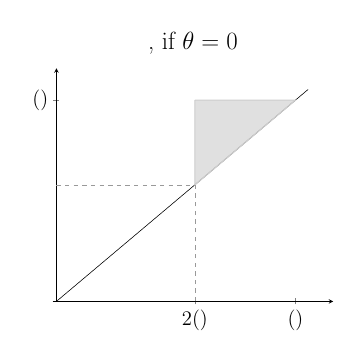
\begin{tikzpicture}[scale=0.52]
	\begin{axis} [
		title={\LARGE $\thetabarc{\cM}$, if $\img\theta_{\cM}= 0$},
		ticklabel style = {font=\Large},
		axis y line=middle,
		axis x line=middle,
		ytick={0.95},
		yticklabels={$\diam(\cM)$},
		xtick={0.55,0.95},
		xticklabels={$2\crit(\cM)$, $\diam(\cM)$},
		xmin=-0.015, xmax=1.1,
		ymin=0, ymax=1.1,]
		\addplot [mark=none] coordinates {(0,0) (1,1)};
		\addplot [thick,color=black!20!white,fill=black!30!white,
		fill opacity=0.4]coordinates {
			(0.55,0.95)
			(0.55,0.55)
			(0.95,0.95)
			(0.55,0.95)};
		\addplot [black!40!white,mark=none,dashed, thin] coordinates {(0,0.55) (0.55,0.55)};
		\addplot [black!40!white,mark=none,dashed, thin] coordinates {(0.55,0) (0.55,0.55)};
	\end{axis}
\end{tikzpicture}
	\caption{In each figure, the gray region represents where additional bars could potentially exist within the corresponding barcode.}
	\label{fig:barcodes_general}
\end{figure}